\documentclass{beamer}

% =====================================================================
% Mesmo molde da apresentação do TCC 1, com o que foi FEITO no TCC 2.
% Tempo (20 min): Introdução 2:30 | Referencial 2:00 | Proposta e Metodologia 3:30 |
% Resultados 8:00 (inclui vídeo de 2:00) | Considerações Finais 2:00 | folga 2:00
% =====================================================================

\mode<presentation>
{
  \usetheme{Berlin}
  \usecolortheme{lily}
  \usefonttheme{professionalfonts}
  \setbeamertemplate{navigation symbols}{}
  \setbeamertemplate{caption}[numbered]
 \setbeamertemplate{bibliography item}[text]
}
\usepackage[T1]{fontenc}
\usepackage{ragged2e}
\usepackage{multirow}
\usepackage{tabularx}
\usepackage{booktabs}
\justifying
\centering

\usepackage[brazil]{babel}
\usepackage[utf8x]{inputenc}
\usepackage{xcolor}

\title[TFG Sistemas de Informação]{
\includegraphics[height=1.9cm]{images/apresentacao/logoUFN-branco.png}\\Sistema Web de Recomendação para Formação de Equipes em Projetos de Desenvolvimento de Software}
\author{Aluno: Eduardo Requia Souza, Orientador: Prof. Alexandre Zamberlan}
\date{UFN - Universidade Franciscana}

\logo{
\includegraphics[height=1cm]{images/logo_si.png}}

\AtBeginSection[]
{
  \begin{frame}<beamer>
    \frametitle{Sumário}
     \tableofcontents[currentsection,currentsubsection]
  \end{frame}
}

\begin{document}

\begin{frame}
  \titlepage
\end{frame}

% =====================================================================
\section{Introdução}
\begin{frame}{Introdução}
    \begin{itemize}
        \item O sucesso de um projeto de software depende da alocação da equipe (impacta qualidade, custos e prazos).
        \item A montagem manual e empírica pelos gestores costuma gerar times desbalanceados, com falta ou sobreposição de habilidades.
        \item Sistemas de Recomendação atuam como Sistemas de Apoio à Decisão, utilizando aprendizado de máquina para otimizar combinações.
        \item Integração de Modelos de Linguagem (LLMs) para tornar as recomendações interpretáveis aos usuários.
    \end{itemize}
\end{frame}

\begin{frame}{Justificativa}
    \begin{itemize}
        \item A alocação inadequada aumenta falhas, atrasa o cronograma e sobrecarrega os profissionais mais experientes.
        \item Analisar de forma estruturada \textit{hard skills}, \textit{soft skills}, senioridade e disponibilidade.
        \item Utilizar algoritmos preditivos para estruturar as decisões do gestor.
        \item Tornar o sistema transparente e interativo através de IA Generativa.
    \end{itemize}
\end{frame}

\begin{frame}[allowframebreaks]{Objetivos}
    \begin{block}{Geral}
     Projetar, implementar e avaliar um protótipo Web de \textcolor{blue}{recomendação de equipes} equilibradas, utilizando modelos de predição e uma \textcolor{blue}{interface conversacional} baseada em IA generativa.
    \end{block}

    \vspace{0.3cm}
    \raggedright Como objetivos \textcolor{blue}{específicos}, assume-se:

    \begin{itemize}
        \item Revisar a bibliografia sobre Sistemas de Recomendação, Reconhecimento de Padrões e Interfaces Conversacionais;
        \item Modelar a estrutura relacional de dados (competências, perfis e requisitos de projetos);
        \item Treinar e avaliar algoritmos de predição em Python para o cálculo de afinidade e ranqueamento de candidatos;
        \item Implementar a integração com o LLM (Gemini) como interface conversacional;
        \item Definir e aplicar cenários controlados de alocação de equipes, validando a coerência técnica do protótipo.
    \end{itemize}
\end{frame}

% =====================================================================
\section{Referencial Teórico}
\begin{frame}{Mapa mental - tópicos}
    \begin{figure}[!ht]
        \centering
        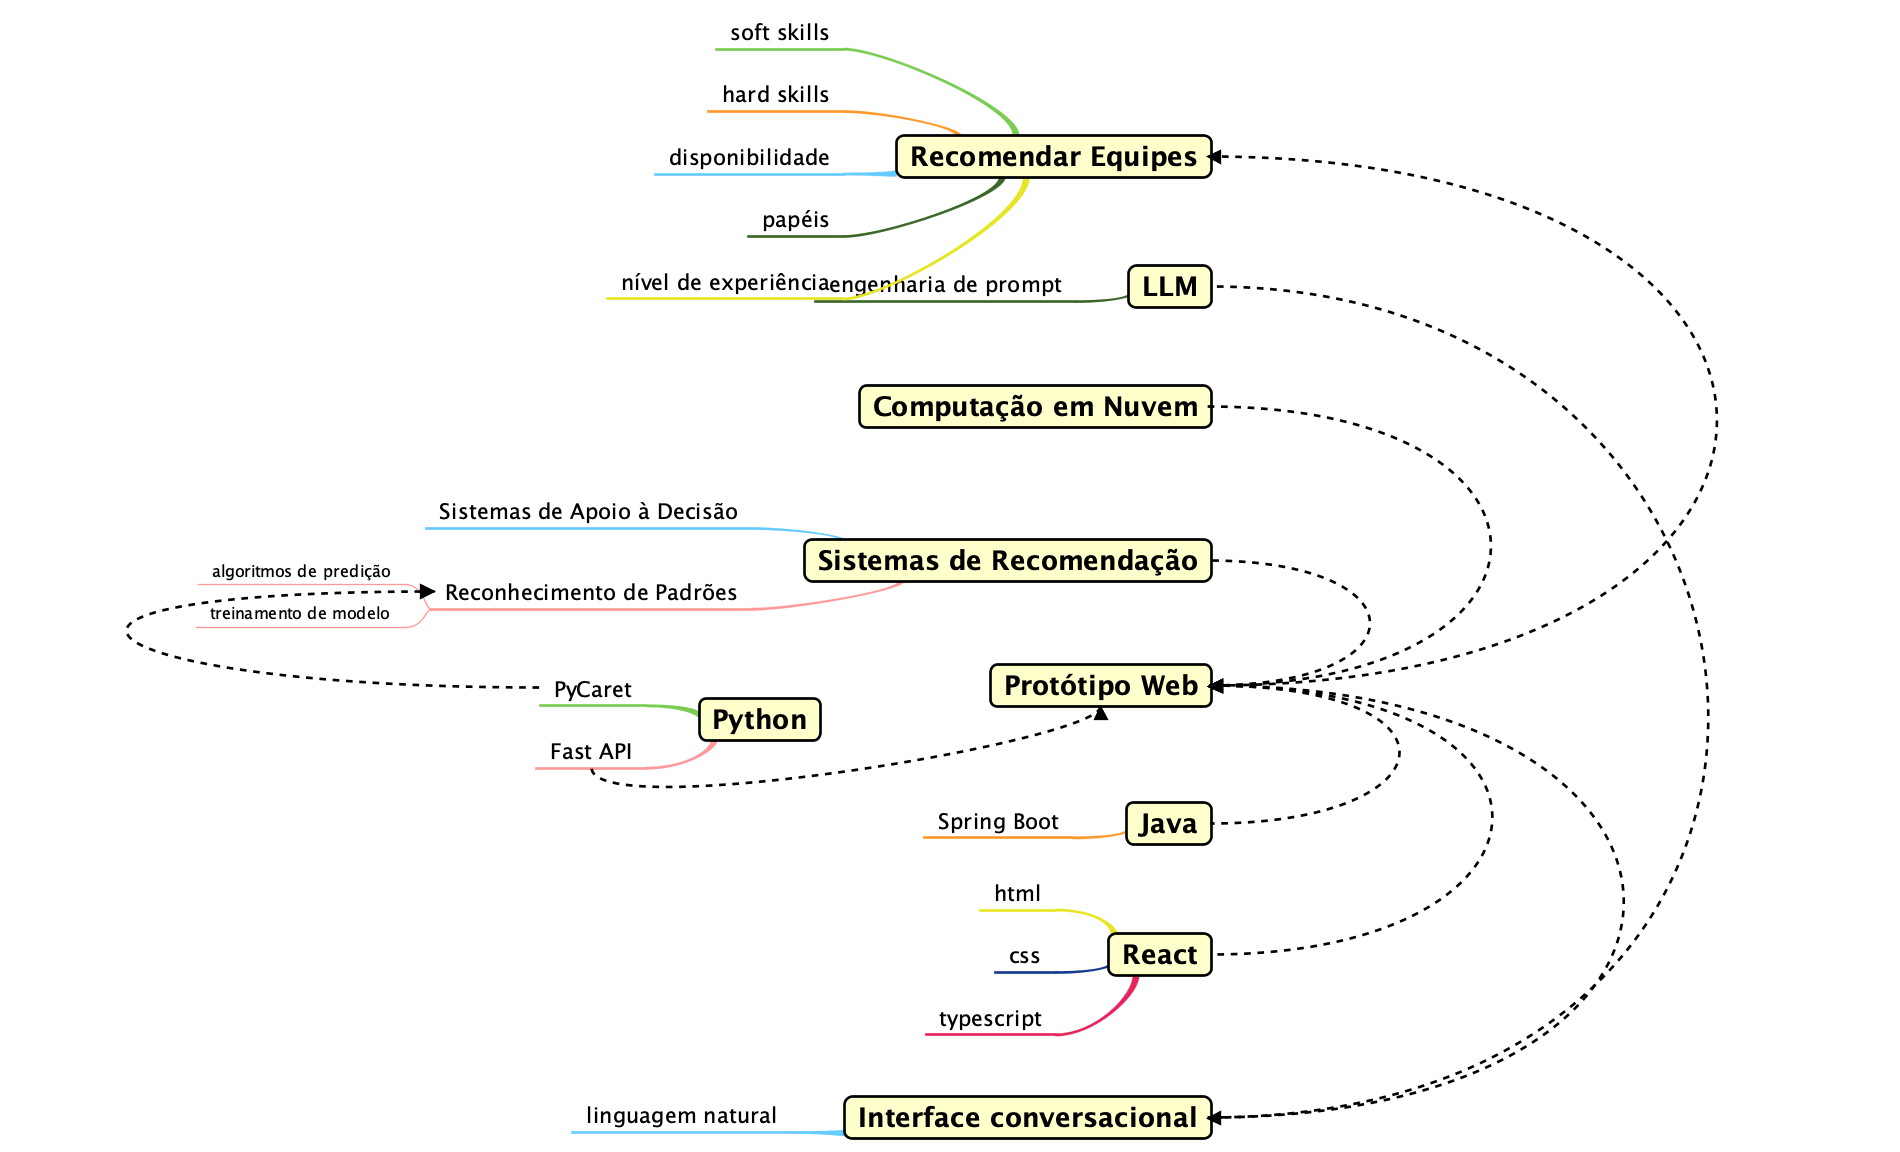
\includegraphics[width=\textwidth,height=0.75\textheight,keepaspectratio]{images/mapaMentalEduardo.png}
        \caption{Conceitos centrais do estudo.}
        \label{fig:mapaMental}
    \end{figure}
\end{frame}

\begin{frame}[allowframebreaks]{Fundamentação}
    \begin{block}{Reconhecimento de Padrões e Engenharia de Atributos}
        Os dados qualitativos dos profissionais são convertidos em variáveis numéricas:
        \begin{itemize}
            \item \textbf{Dados Ordinais:} Senioridade (Júnior, Pleno, Sênior) $\rightarrow$ 1, 2, 3;
            \item \textbf{Dados Nominais:} Papéis de atuação (\textit{Backend}, \textit{Frontend}, ...) $\rightarrow$ vetores binários;
            \item \textbf{Dados Contínuos:} Disponibilidade semanal (carga horária).
        \end{itemize}
        O modelo gera um \textcolor{blue}{escore de afinidade} entre profissional e projeto.
    \end{block}

    \framebreak

    \begin{block}{LLMs e Interfaces Conversacionais (Dupla Via)}
        \begin{itemize}
            \item Algoritmos de predição clássicos geram cálculos exatos, mas carecem de transparência e de interação em linguagem natural.
            \item \textbf{Via de Entrada:} O gestor descreve a equipe em linguagem natural e o LLM extrai os parâmetros da recomendação.
            \item \textbf{Via de Saída:} O Gemini recebe os dados do ranqueamento e redige a justificativa da equipe.
        \end{itemize}
    \end{block}
\end{frame}

% =====================================================================
\section{Proposta e Metodologia}
\begin{frame}{Metodologia}

    \raggedright \textbf{Pesquisa exploratória}, com revisão bibliográfica e \textbf{estudo de caso}, em arquitetura de \textbf{microsserviços}.

    \begin{itemize}
        \item \textcolor{blue}{Scrum} customizado e gestão visual via \textcolor{blue}{Kanban};
        \item \textcolor{blue}{GitHub} para controle de versionamento do código;
        \item \textbf{Frontend:} Interface desenvolvida em \textcolor{blue}{React};
        \item \textbf{Backend:} \textcolor{blue}{Java 21}, \textcolor{blue}{Spring Boot 3} e PostgreSQL;
        \item \textbf{Motor Preditivo:} \textcolor{blue}{Python 3.10, FastAPI} e \textcolor{blue}{PyCaret} (LightGBM);
        \item \textbf{IA Generativa:} \textcolor{blue}{Spring AI} integrando a API do \textcolor{blue}{Google Gemini}.
    \end{itemize}
 \end{frame}

\begin{frame}[allowframebreaks]{Modelagem}
\raggedright \textbf{Abordagem Híbrida de Interação}
\begin{itemize}
    \item \textbf{Via Formulários:} Entrada de dados estruturada (JSON) diretamente no \textit{Backend}.
    \item \textbf{Via Interface Conversacional:} O LLM extrai os parâmetros do pedido do gestor na entrada e justifica a formação da equipe na saída.
\end{itemize}

\framebreak

\begin{figure}[!h]
\centering
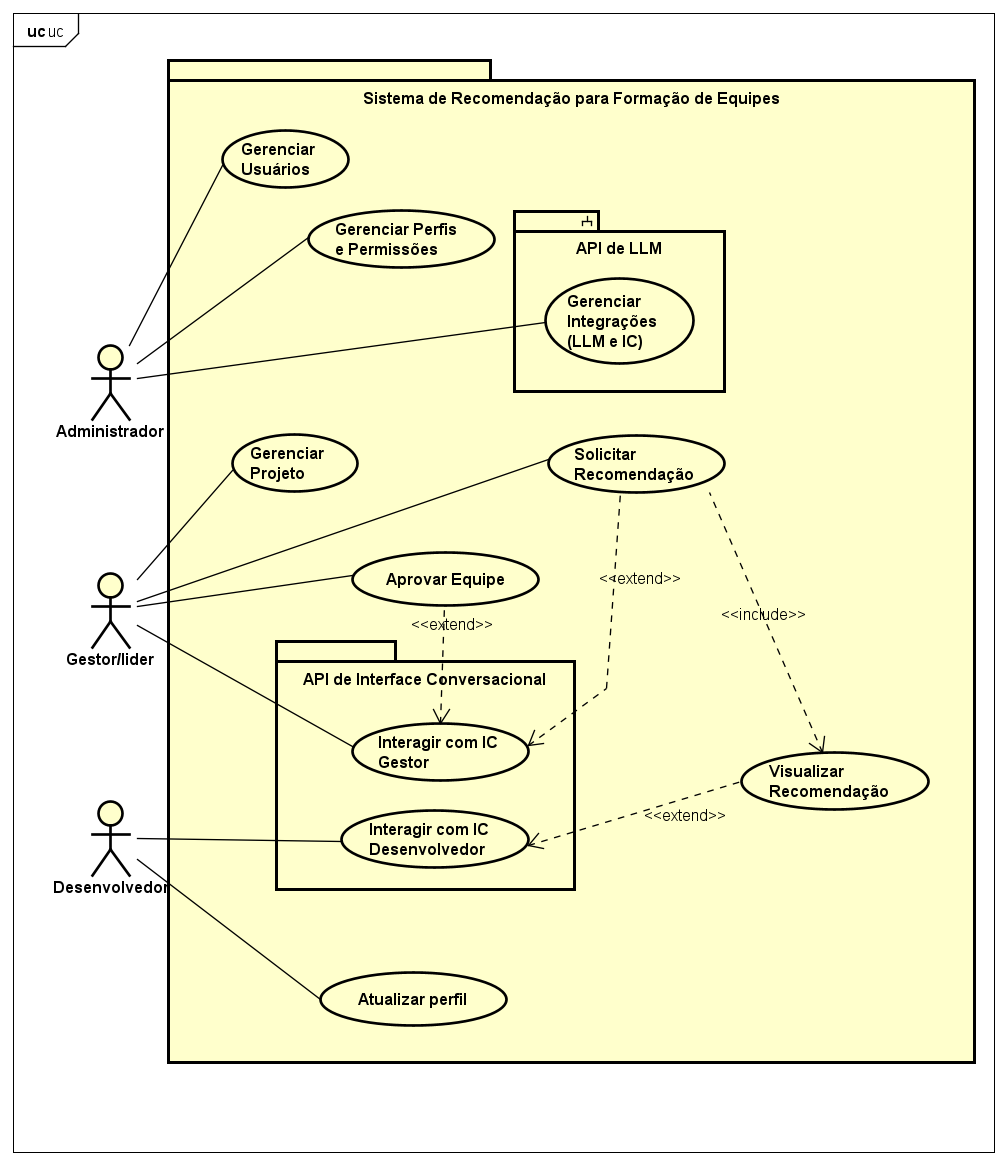
\includegraphics[width=\textwidth,height=0.7\textheight,keepaspectratio]{images/casoDeUso_tcc1.png}
\caption{Diagrama de Casos de Uso detalhando a dupla via de interação.}
\label{fig:casoDeUso}
\end{figure}

\framebreak

\begin{figure}[!ht]
\centering
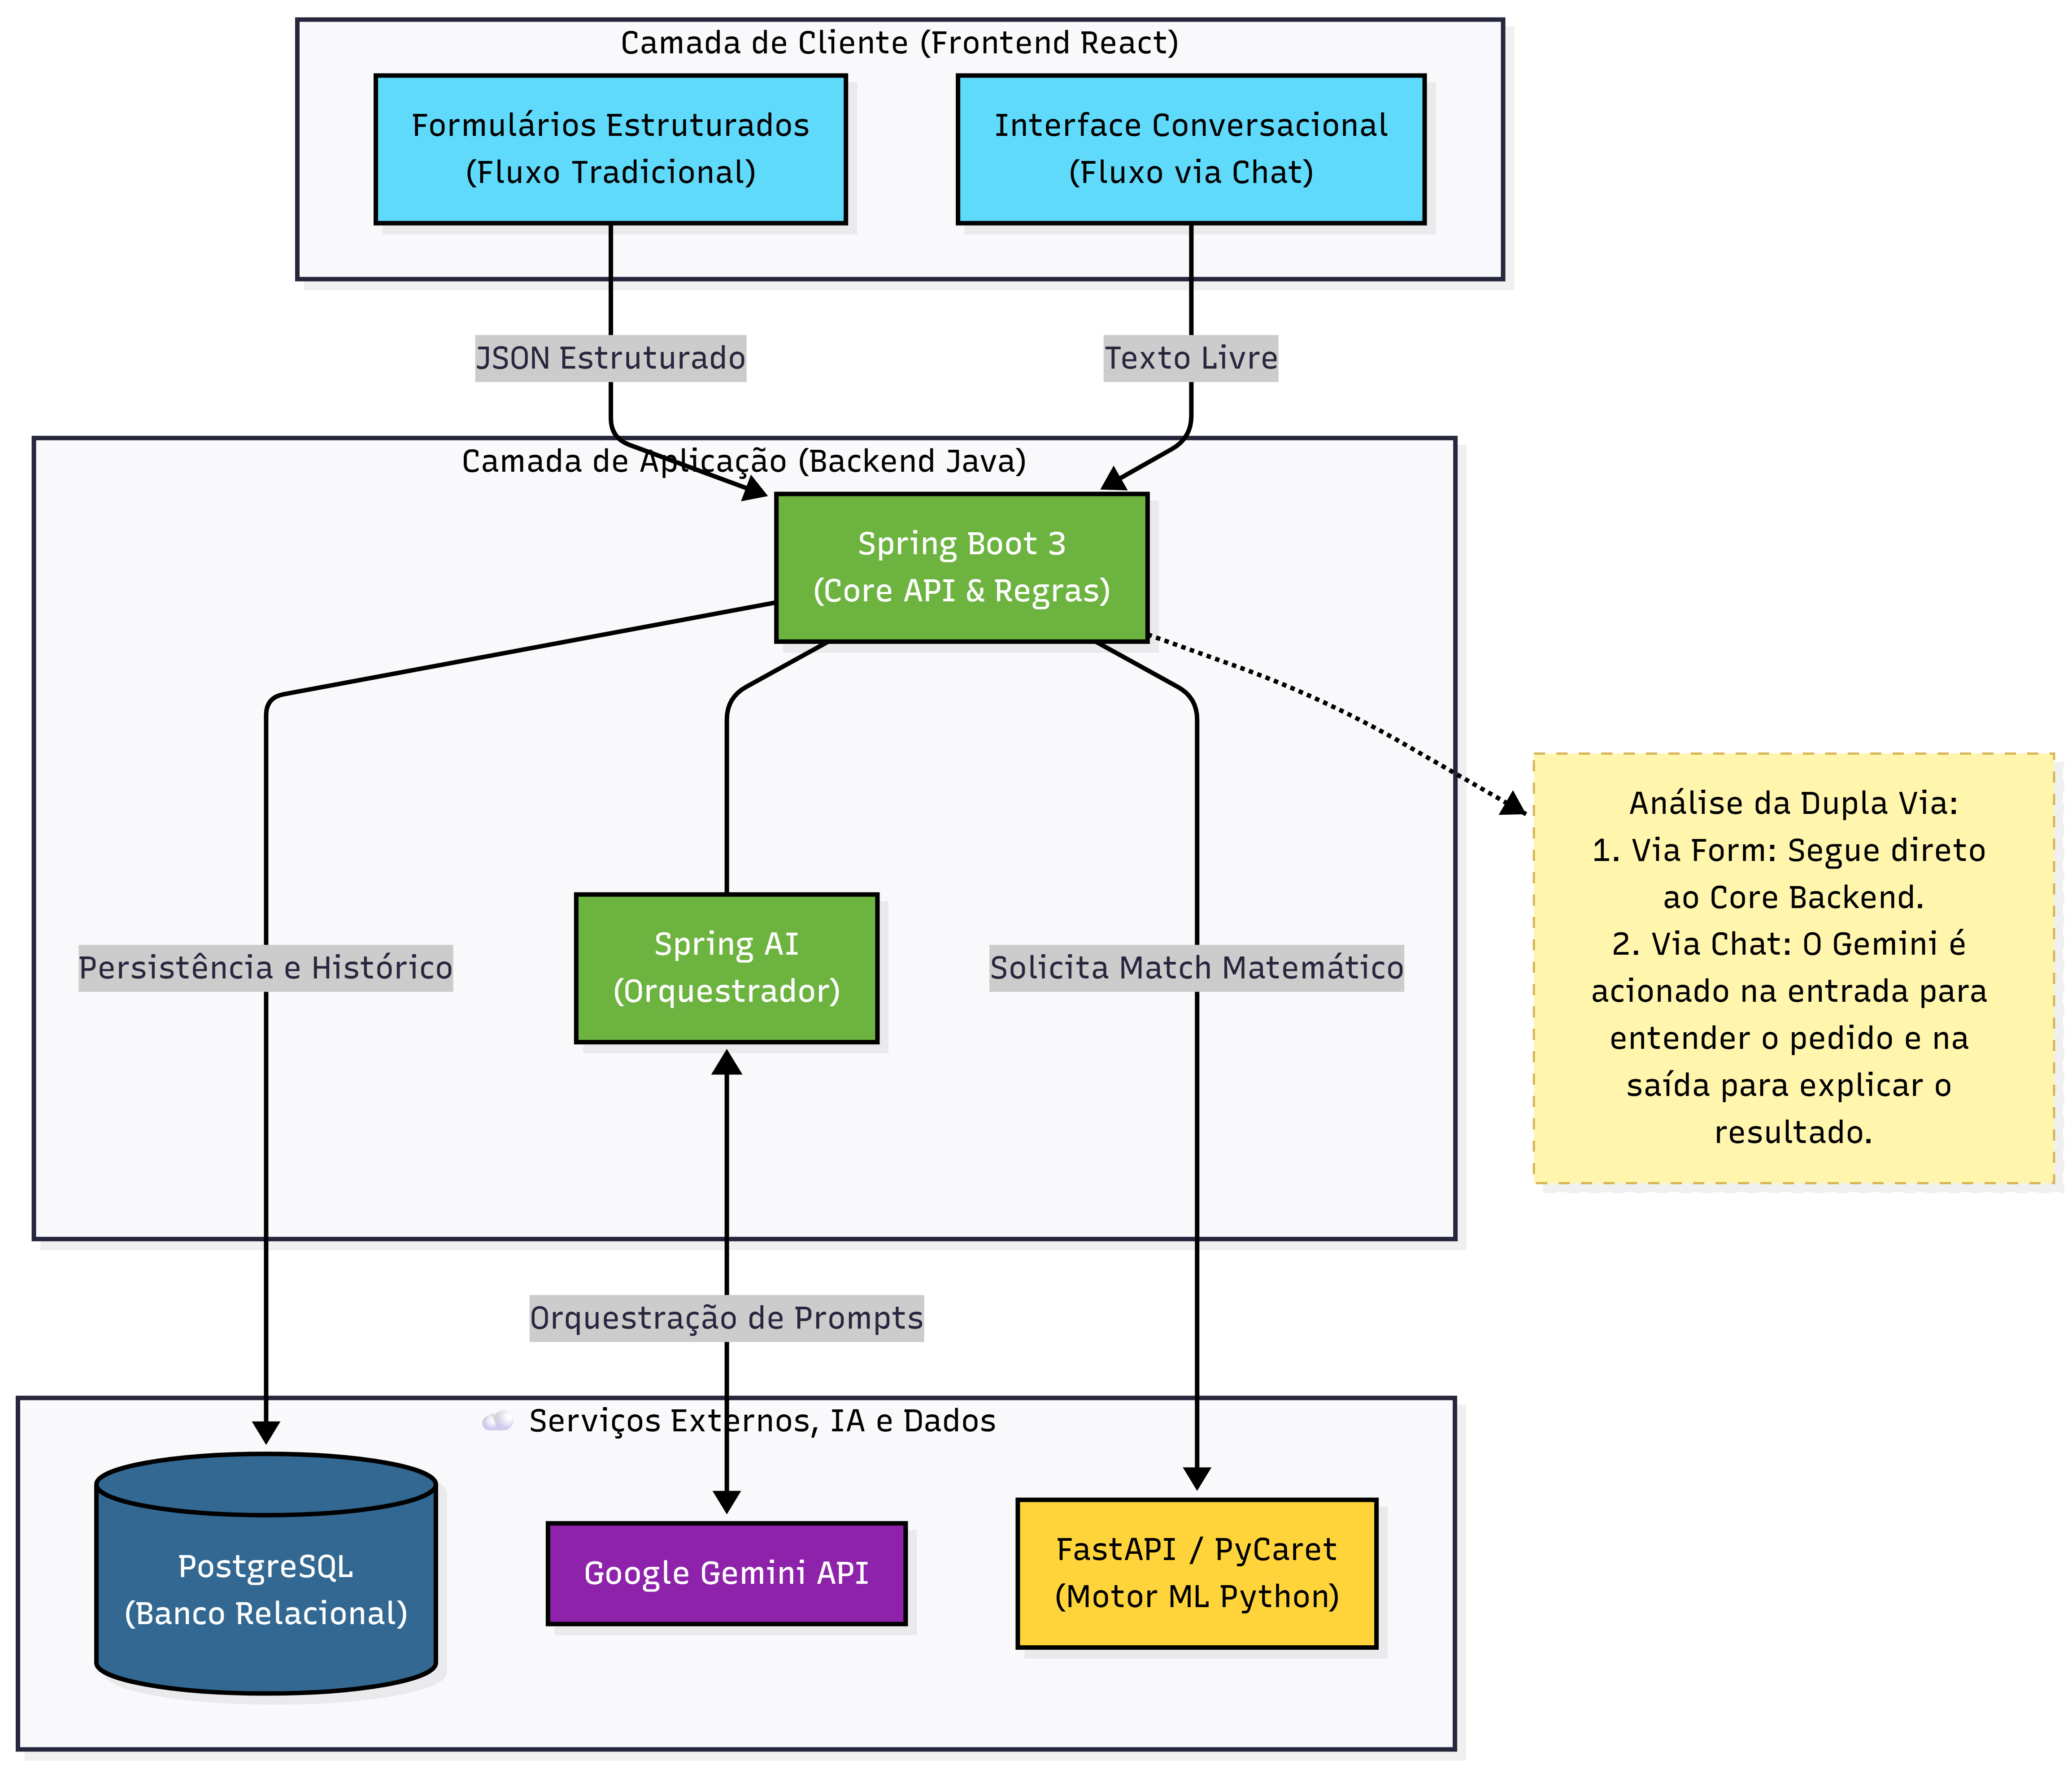
\includegraphics[width=\textwidth,height=0.6\textheight,keepaspectratio]{images/diagComponentes2.png}
\caption{Diagrama de Componentes integrando Spring Boot, FastAPI e Gemini.}
\label{fig:diagComponentes}
\end{figure}

\end{frame}

\begin{frame}[allowframebreaks]{Estudo de caso e Cenários}

\raggedright \textbf{Cenários de Avaliação} (executados no protótipo em funcionamento):
\begin{enumerate}
    \item Papéis mínimos obrigatórios;
    \item Balanceamento de experiência (criticidade alta);
    \item Escassez de disponibilidade;
    \item Conflito entre projetos simultâneos.
\end{enumerate}

\vspace{0.2cm}
\raggedright \textbf{Linha de base:} 100 equipes sorteadas (semente fixa) entre os \textcolor{blue}{mesmos elegíveis}.

\framebreak

\raggedright \textbf{Métricas da equipe proposta:}
\begin{itemize}
    \item \textbf{Cobertura de papéis:} \% das vagas preenchidas pelo papel exigido;
    \item \textbf{Cobertura de tecnologias:}
    \[ CT = \frac{\sum_{t \in D} p_t}{\sum_{t \in E} p_t} \times 100 \]
    $E$: tecnologias exigidas; $D$: dominadas por ao menos um integrante; $p_t$: peso;
    \item \textbf{Dispersão} ($\sigma_s$): desvio padrão da senioridade;
    \item \textbf{Escore médio} de afinidade da equipe.
\end{itemize}

\end{frame}

% =====================================================================
\section[Resultados]{Resultados e Discussões}

% Telas: mostrar rápido, o vídeo detalha.
\begin{frame}[allowframebreaks]{Protótipo}
    \begin{figure}[!ht]
        \centering
        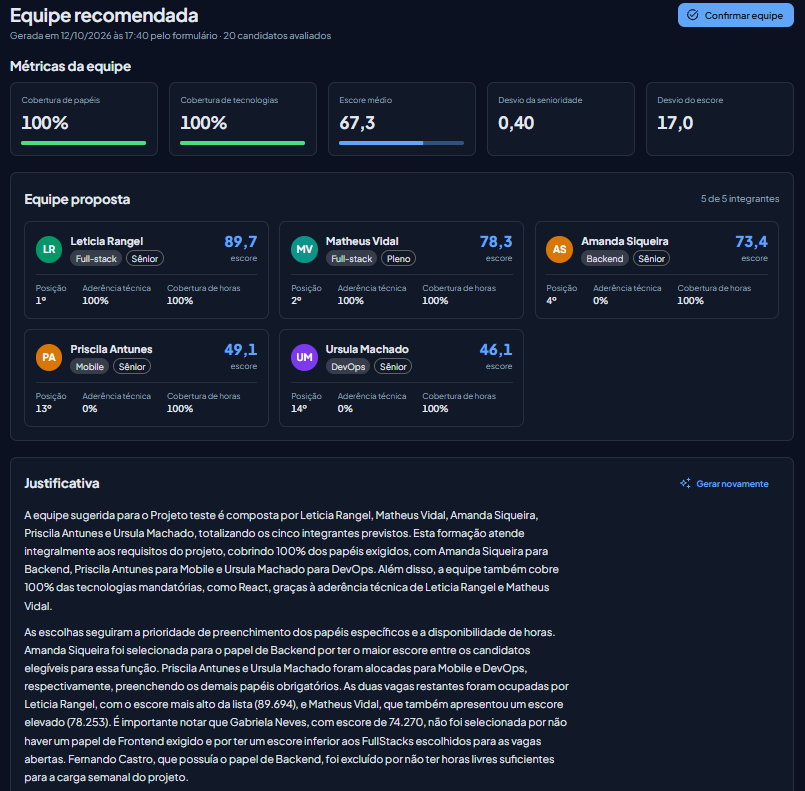
\includegraphics[width=\textwidth,height=0.7\textheight,keepaspectratio]{images/telaRecomendacao.png}
        \caption{Ranqueamento, composição da equipe e justificativa gerada pelo LLM.}
    \end{figure}

    \framebreak

    \begin{figure}[!ht]
        \centering
        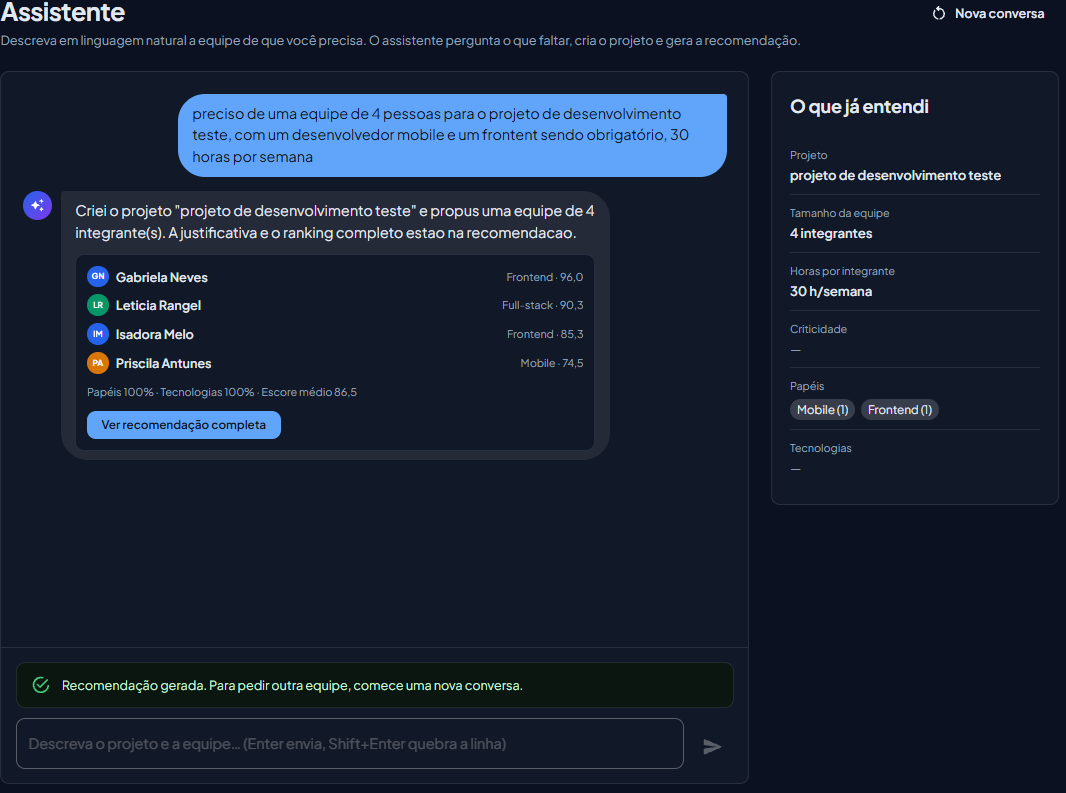
\includegraphics[width=\textwidth,height=0.7\textheight,keepaspectratio]{images/telaAssistente.png}
        \caption{Interface conversacional: pedido em linguagem natural.}
    \end{figure}
\end{frame}

\begin{frame}[allowframebreaks]{Motor Preditivo}
    \raggedright \textbf{Base de dados}
    \begin{itemize}
        \item \textcolor{blue}{Stack Overflow Developer Survey 2024}: 33.462 profissionais (\textit{backend}, \textit{frontend}, \textit{fullstack}, \textit{mobile}, QA, DevOps);
        \item \textit{Soft skills} (0 a 5) e disponibilidade (0 a 60 h) geradas sinteticamente;
        \item Perfis cruzados com projetos fictícios de criticidade baixa, média e alta;
        \item Variável alvo: \textbf{escore de afinidade} (0 a 100), pela regra abaixo + ruído.
    \end{itemize}
    \begin{table}
        \scriptsize
        \caption{Pesos de cada componente do escore conforme a criticidade.}
        \resizebox{\textwidth}{!}{\begin{tabular}{lccccc}
            \toprule
            Criticidade & Papel & Técnica & Senioridade & Comportamental & Disponibilidade \\
            \midrule
            Baixa (1) & 25 & 30 & 15 & 15 & 15 \\
            Média (2) & 25 & 25 & 20 & 15 & 15 \\
            Alta (3)  & 25 & 15 & 25 & 20 & 15 \\
            \bottomrule
        \end{tabular}}
    \end{table}

    \framebreak

    \raggedright 13 variáveis; 80\% treino / 20\% teste; validação cruzada em 10 partições; \textbf{regressão}.
    \begin{table}
        \caption{Comparação entre os algoritmos de regressão no PyCaret.}
        \resizebox{\textwidth}{!}{\begin{tabular}{lrrrrrr}
            \toprule
            Algoritmo & MAE & MSE & RMSE & R\textsuperscript{2} & MAPE & Tempo (s) \\
            \midrule
            \textcolor{blue}{\textbf{Light Gradient Boosting Machine}} & \textbf{3,3278} & \textbf{17,4363} & \textbf{4,1755} & \textbf{0,9333} & \textbf{0,0664} & 0,93 \\
            Extreme Gradient Boosting & 3,4840 & 19,0565 & 4,3649 & 0,9271 & 0,0664 & 0,31 \\
            Random Forest & 3,7258 & 21,8543 & 4,6745 & 0,9164 & 0,0740 & 7,42 \\
            Extra Trees & 3,7475 & 22,1576 & 4,7070 & 0,9153 & 0,0737 & 6,41 \\
            Gradient Boosting & 3,7653 & 22,4450 & 4,7369 & 0,9142 & 0,0771 & 1,60 \\
            K Neighbors & 4,0463 & 26,5490 & 5,1521 & 0,8985 & 0,0886 & 0,24 \\
            Decision Tree & 5,0378 & 40,8181 & 6,3885 & 0,8439 & 0,0991 & 0,12 \\
            Linear Regression & 5,9475 & 59,0299 & 7,6819 & 0,7743 & 0,1209 & 1,14 \\
            AdaBoost & 7,8417 & 90,3780 & 9,5060 & 0,6545 & 0,1654 & 1,13 \\
            Passive Aggressive & 7,6746 & 92,1845 & 9,5329 & 0,6470 & 0,1472 & 0,07 \\
            Lasso Regression & 8,5388 & 111,7844 & 10,5720 & 0,5727 & 0,1904 & 0,04 \\
            Elastic Net & 10,4065 & 166,0893 & 12,8868 & 0,3652 & 0,2365 & 0,04 \\
            Orthogonal Matching Pursuit & 11,2313 & 193,8303 & 13,9219 & 0,2590 & 0,2515 & 0,04 \\
            Dummy Regressor & 13,1271 & 261,7599 & 16,1780 & $-$0,0004 & 0,3008 & 0,03 \\
            \bottomrule
        \end{tabular}}
    \end{table}
    \scriptsize \textbf{MAE}: erro médio em pontos (0--100); \textbf{RMSE}: penaliza erros grandes; \textbf{R\textsuperscript{2}}: proporção da variação do escore explicada (1 = perfeito).

    \framebreak

    \begin{itemize}
        \item O \textcolor{blue}{LightGBM} obteve o melhor resultado em todas as métricas de erro (empate com XGBoost no MAPE).
        \item Os cinco primeiros são baseados em árvores: capturam interações como ``senioridade vale mais em projetos críticos''; a regressão linear não passou de R\textsuperscript{2} = 0,77.
        \item Comparado à regra sem ruído em 3.000 combinações novas: erro médio de \textbf{1,08 ponto}.
    \end{itemize}
\end{frame}

\begin{frame}[allowframebreaks]{Aplicação do Modelo na Recomendação}
    \begin{table}
        \caption{Obtenção das variáveis de entrada do modelo a partir dos dados do sistema.}
        \resizebox{\textwidth}{!}{\begin{tabular}{lll}
            \toprule
            Variável & Origem no sistema & Cálculo \\
            \midrule
            Senioridade & Cadastro do desenvolvedor & Júnior = 1, Pleno = 2, Sênior = 3 \\
            Papéis de atuação (6) & Papel principal do desenvolvedor & 1 no papel do desenvolvedor e 0 nos demais \\
            Competências comportamentais & Cadastro do desenvolvedor & Valor direto, de 0 a 5 \\
            Criticidade & Cadastro do projeto & Baixa = 1, Média = 2, Alta = 3 \\
            Requisito de backend & Papéis exigidos pelo projeto & 1 se o projeto exige backend ou fullstack \\
            Requisito de frontend & Papéis exigidos pelo projeto & 1 se o projeto exige frontend ou fullstack \\
            Aderência técnica & Tecnologias do desenvolvedor e do projeto & Pesos das tecnologias dominadas $\div$ pesos exigidos \\
            Cobertura de horas & Disponibilidade, alocações e projeto & Horas livres $\div$ horas exigidas, limitada a 1 \\
            \bottomrule
        \end{tabular}}
    \end{table}

    \framebreak

    \raggedright \textbf{Composição da equipe} (aplicada pelo \textit{backend} sobre o ranqueamento):
    \begin{enumerate}
        \item \textbf{Elegibilidade:} só entra quem tem horas livres suficientes;
        \item \textbf{Vagas por papel:} elegível de maior escore com aquele papel;
        \item \textbf{Posições livres:} maiores escores restantes.
    \end{enumerate}
    \begin{itemize}
        \item Faltando elegíveis, propõe a melhor equipe possível e registra as restrições;
        \item Horas descontadas só quando o gestor \textcolor{blue}{confirma} a equipe.
    \end{itemize}
\end{frame}

% VÍDEO (2:00), só a recomendação:
%  0:00-0:20  projeto já cadastrado: criticidade, horas, papéis e tecnologias exigidas
%  0:20-1:05  gerar recomendação: ranking, escores, equipe e um inelegível por horas
%  1:05-1:40  métricas da equipe e justificativa do Gemini
%  1:40-2:00  confirmar a equipe (horas descontadas)
\begin{frame}{Demonstração do Protótipo}
    \centering
    \vfill
    {\Large \textcolor{blue}{Recomendação de equipe}}\\[1em]
    (vídeo)
    \vfill
\end{frame}

\begin{frame}[allowframebreaks]{Cenários de Avaliação}
    \begin{table}
        \caption{Resultados dos cenários de avaliação.}
        \resizebox{\textwidth}{!}{\begin{tabular}{clcccc}
            \toprule
            Cenário & Equipe & Papéis (\%) & Tecnologias (\%) & $\sigma_s$ & Escore médio \\
            \midrule
            \multirow{2}{*}{1} & \textcolor{blue}{\textbf{Protótipo}} & \textbf{100,00} & \textbf{100,00} & \textbf{0,490} & \textbf{69,674} \\
              & Linha de base & 59,60 $\pm$ 16,97 & 93,84 $\pm$ 8,52 & 0,702 $\pm$ 0,148 & 62,882 $\pm$ 5,690 \\
            \midrule
            \multirow{2}{*}{2} & \textcolor{blue}{\textbf{Protótipo}} & \textbf{100,00} & \textbf{100,00} & \textbf{0,000} & \textbf{86,491} \\
              & Linha de base & 78,33 $\pm$ 20,21 & 88,37 $\pm$ 11,05 & 0,631 $\pm$ 0,251 & 61,474 $\pm$ 7,625 \\
            \midrule
            3 & Protótipo = linha de base (3/5) & 60,00 & 100,00 & 0,471 & 73,958 \\
            \midrule
            \multirow{2}{*}{4} & Projeto A & 100,00 & 100,00 & 0,000 & 85,952 \\
              & Projeto B, após confirmar A & 100,00 & 84,21 & 0,000 & 68,518 \\
            \bottomrule
        \end{tabular}}
    \end{table}

    \framebreak

    \begin{itemize}
        \item \textbf{Cenário 1:} 100\% dos papéis contra 59,60\% dos sorteios; o QA (escore 45,98) entrou e a \textit{fullstack} sênior (88,03) ficou de fora, pois a vaga de QA era exigida.
        \item \textbf{Cenário 2:} os quatro sêniores no topo; dispersão nula e escore médio cerca de 3,3 desvios padrão dos sorteios acima da média.
        \item \textbf{Cenário 3:} apenas 3 de 14 com horas; equipe parcial com as restrições registradas.
        \item \textbf{Cenário 4:} confirmado o Projeto A, o Projeto B recebeu 4 profissionais distintos, sem sobreposição; a tecnologia caiu para 84,21\%.
    \end{itemize}
\end{frame}

% =====================================================================
\section{Considerações Finais}
\begin{frame}[allowframebreaks]{Considerações Finais}
    \begin{block}{O que foi realizado (TCC 2)}
    \begin{itemize}
        \item Protótipo implementado: interfaces em React, \textit{backend} em Spring Boot, motor preditivo em Python e interface conversacional com o Gemini;
        \vspace{0.2cm}

        \item Motor preditivo treinado e avaliado: o \textcolor{blue}{LightGBM} obteve o melhor desempenho (R\textsuperscript{2} = 0,93);
        \vspace{0.2cm}

        \item Nos cenários com escolha, o protótipo superou a composição aleatória em todas as métricas; sob restrições, propõe equipes parciais e evita sobreposição entre projetos.
    \end{itemize}
    \end{block}

    \framebreak

    \begin{block}{Limitações}
        Variável alvo e parte dos atributos sintéticos; perfis fictícios nos cenários. As conclusões se restringem à validação técnica.
    \end{block}

    \begin{block}{Trabalhos Futuros}
        \begin{itemize}
            \item Aplicação em ambiente organizacional, com histórico real de alocações e desfechos;
            \item Realimentação do modelo com as avaliações do gestor;
            \item Otimização combinatória da equipe como um todo.
        \end{itemize}
    \end{block}

\end{frame}

% =====================================================================
\section{Referências}
\begin{frame}[allowframebreaks]{Referências}
    \nocite{*}
    \bibliographystyle{IEEEtran}
    \bibliography{references}
\end{frame}

\end{document}
